\begin{figure}[ht]
    \centering
    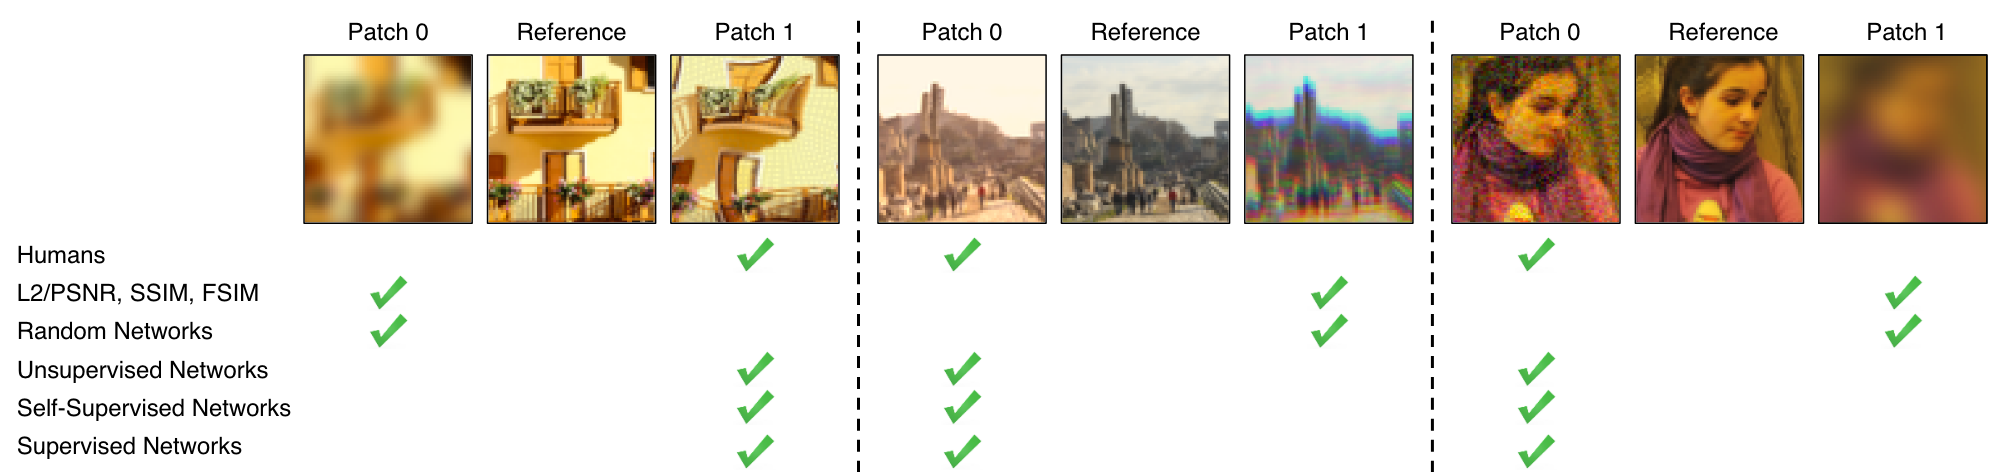
\includegraphics[width=1.0\textwidth]{figures/lpips.png}
    \caption{Figure 1 from LPIPS \cite{zhang_unreasonable_2018}. LPIPS is trained to perceive image similarity the same way humans do. The dataset used to train the similarity metric contains two types of perceptual judgements, Two Alternative Forced Choice (\pmb{2AFC}) and Just Noticeable Differences (\pmb{JND}). With 2AFC people were asked to select which of the distorted images was "closer" to the reference. With JND people were presented with 2 image patches, one reference and one distorted, and asked if they were the same.}
    \label{fig:lpips}
\end{figure}